\documentclass[10pt]{beamer}
\usepackage{beamerthemeblackboard}
\usepackage{graphics}
%\usepackage{emerald}
%\usepackage[T1]{fontenc}
\usepackage{amsmath,amsthm,amsfonts,latexsym,amscd,amssymb,xcolor,enumerate,hyperref,pifont}
%\usepgfplotslibrary{dateplot}
\usepackage{graphicx}
\usepackage{pdftricks}
\input{xypic}
\usepackage{psfrag}
\usepackage{rotating}
\usepackage{multirow}
\usepackage[thicklines]{cancel}
\renewcommand\CancelColor{\color{orange}}
\usepackage{graphicx}


%\includeonlyframes{current}

\usepackage{csquotes}
\usepackage{tcolorbox}\usepackage{mdframed}
\begin{psinputs}
 \usepackage[usenames,dvipsnames]{pstricks}
 \usepackage{epsfig}
  \usepackage{pst-grad} % For gradients
 \usepackage{pst-plot} % For axes
\end{psinputs}
%\usepackage{xcolor}
\usepackage{tikz}
\usepackage{subcaption}
\usepackage{mathtools}

\usetikzlibrary{arrows,shapes}
\usepackage{animate}
\usepackage{calc}

\usepackage{colortbl}



%\definecolor{light-gray}{gray}{0.80}
%\usecolortheme{beaver}
% User Defined Operators
%%%%%%%
\newtheorem{rem}[theorem]{Remark}
%\newtheorem{facts}[theorem]{facts}
\newtheorem{proposition}[theorem]{Proposition}
%\DeclareMathOperator{\dim}{dim}
\newcommand{\DIFF}{\mathrm{DIFF}}
\newcommand{\TOP}{\mathrm{TOP}} 
\newcommand{\ORB}{\mathrm{ORB}}
\newcommand{\ALEX}{\mathrm{ALEX}}
%%%%%%%%%%%%

%Operators
\DeclareMathOperator{\rank}{rank}
\DeclareMathOperator{\Susp}{Susp}
\DeclareMathOperator{\curv}{curv}
\DeclareMathOperator{\fix}{Fix}
\DeclareMathOperator{\Isom}{Isom}


%%%%%%%%%%%%%%%%%%%%%%%%
% Draw Line below Frametitle

\newcommand{\topline}{%
  \tikz[remember picture,overlay] {%
    \draw[white] ([yshift=-1.6cm,xshift=0.9cm]current page.north west)
             -- ([yshift=-1.6cm,xshift=11cm]current page.north west);}}
%%%%%%%%%%%%%%%%%%%%%%%

%THEOREMS
%\newtheorem{fact}[thm]{Fact}
%%%%%%%%%%%%%%%%%%%%%%%


%TIKZ
\newcommand\pgfmathsinandcos[3]{%
  \pgfmathsetmacro#1{sin(#3)}%
  \pgfmathsetmacro#2{cos(#3)}%
}
\newcommand\LongitudePlane[3][current plane]{%
  \pgfmathsinandcos\sinEl\cosEl{#2} % elevation
  \pgfmathsinandcos\sint\cost{#3} % azimuth
  \tikzset{#1/.style={cm={\cost,\sint*\sinEl,0,\cosEl,(0,0)}}}
}
\newcommand\LatitudePlane[3][current plane]{%
  \pgfmathsinandcos\sinEl\cosEl{#2} % elevation
  \pgfmathsinandcos\sint\cost{#3} % latitude
  \pgfmathsetmacro\yshift{\cosEl*\sint}
  \tikzset{#1/.style={cm={\cost,0,0,\cost*\sinEl,(0,\yshift)}}} %
}
\newcommand\DrawLongitudeCircle[2][1]{
  \LongitudePlane{\angEl}{#2}
  \tikzset{current plane/.prefix style={scale=#1}}
   % angle of "visibility"
  \pgfmathsetmacro\angVis{atan(sin(#2)*cos(\angEl)/sin(\angEl))} %
  \draw[current plane] (\angVis:1) arc (\angVis:\angVis+180:1);
  \draw[current plane,dashed] (\angVis-180:1) arc (\angVis-180:\angVis:1);
}
\newcommand\DrawLatitudeCircle[2][2]{
  \LatitudePlane{\angEl}{#2}
  \tikzset{current plane/.prefix style={scale=#1}}
  \pgfmathsetmacro\sinVis{sin(#2)/cos(#2)*sin(\angEl)/cos(\angEl)}
  % angle of "visibility"
  \pgfmathsetmacro\angVis{asin(min(1,max(\sinVis,-1)))}
  \draw[current plane] (\angVis:1) arc (\angVis:-\angVis-180:1);
  \draw[current plane,dashed] (180-\angVis:1) arc (180-\angVis:\angVis:1);
}
\usetikzlibrary{quotes,angles,positioning,calc,hobby}
%\usetkzobj{all}
%\usetkzobj{arcs}

%\AtBeginDocument{\ECFAugie}
%% Date in the Corner
%\setbeamertemplate{headline}{
%    \rotatebox{30}{
%        \ifx\insertdate\empty\else        
%            \hspace*{0.25cm}\ECFAugie\insertshortdate\hspace*{0.5cm}
%        \fi
%    }
%    \vspace*{-1cm}
%}
	%\setbeamertemplate{footline} % To remove the footer line in all slides uncomment this line
\setbeamertemplate{footline}[frame number] % To replace the footer line in all slides with a simple slide count uncomment this line



\setbeamertemplate{navigation symbols}{}
\DeclareMathOperator{\dist}{dist}
\DeclareMathOperator{\cone}{Cone}
\DeclareMathOperator{\alex}{Alex}

\newcommand{\bbR}{\mathbb{R}}
\newcommand{\bbP}{\mathbb{P}}
\newcommand{\bbQ}{\mathbb{Q}}
\newcommand{\bbC}{\mathbb{C}}
\newcommand{\bbZ}{\mathbb{Z}}
\newcommand{\ahat}{\hat{\mathcal{A}}}
\newcommand{\Hyp}{\mathbb{H}}
%\newcommand{\Ric}{\mathrm{Ric}}
\DeclareMathOperator{\Ric}{Ric}
\DeclarePairedDelimiter{\scpr}{\langle}{\rangle}
\newcommand{\R}{\mathbb{R}}
\newcommand{\calR}{\mathcal{R}}
\newcommand{\calM}{\mathcal{M}}
\newcommand{\frso}{\mathfrak{so}}
\newcommand{\K}{\mathcal{K}}
\newcommand{\N}{\mathbb{N}} 
\newcommand{\Z}{\mathbb{Z}}
\newcommand{\Qu}{\mathbb{H}} 
\newcommand{\Q}{\mathbb{Q}}
\newcommand{\sing}{\text{sing}} 
\newcommand{\BP}{\rm BP} 
\newcommand{\eps}{\varepsilon}
\definecolor{dred}{rgb}{.6,0,0} 
\definecolor{dgreen}{rgb}{0,.2,0} 
\definecolor{lred}{rgb}{0.9,0,0}
\definecolor{mul}{rgb}{0.5,0,0.5}
\definecolor{dblue}{rgb}{.2,.2,.8} 
\newcommand{\pretendbigger}[1]{\makebox[0pt]{\phantom{\bigg(}}\hspace*{5ex}{#1}\hspace*{5ex}} 
\newcommand{\red}[1]{\textcolor{red}{#1}} 
\newcommand{\green}[1]{\textcolor{green}{#1}} 
\newcommand{\blue}[1]{\textcolor{blue}{#1}} 
\newcommand{\orange}[1]{\textcolor{orange}{#1}} 
\newcommand{\gray}[1]{\textcolor{lightgray}{#1}} 
\newcommand{\psc}{{\mathrm{scal}>0}}
\newcommand{\prc}{{\mathrm{Ric}>0}}
\newcommand{\psec}{{\mathrm{Sec}>0}}
\newcommand{\nsc}{{\mathrm{scal}<0}}
\newcommand{\nnrc}{{\mathrm{Ric}\ge0}}
\newcommand{\zrc}{{\mathrm{Ric}\equiv0}}
\newcommand{\nnsec}{{\mathrm{Sec}\ge0}}
\newcommand{\Spin}{\mathrm{Spin}}
\newcommand{\eucl}{\mathrm{eucl}}
\newcommand{\actson}{\curvearrowright}
\newcommand{\diff}{{\mathrm{Diff}}}

\DeclareMathOperator{\vol}{vol}
\DeclareMathOperator{\scal}{scal}
\DeclareMathOperator{\diam}{diam}
\newcommand{\myicon}{$\,\,\,\triangleright$}

\title{Diffeomorphisms and Positive Scalar Curvature}
\author{Georg Frenck} 
\institute{\small{University of Augsburg}
\vspace{3em}}
\date{{December 21st, 2021}}

\newtheorem*{Thm A}{Theorem A}
\newtheorem*{Thm B}{Theorem B}
\newtheorem*{Conj}{Conjecture}
\newtheorem*{que}{Question}
\newtheorem{defn}{Definition}
\newtheorem*{prop}{Proposition}
\newtheorem*{thm}{Theorem}
\newtheorem{cor}{Corollary}
\newtheorem*{lem}{Lemma}
\newtheorem*{remark}{Remark}

\begin{document}

\begin{frame}[plain]
\maketitle  
\end{frame}


\begin{frame}[plain] 
  \frametitle{Introduction and Motivation}
  \topline 
  \setlength{\fboxsep}{0pt}
  \vspace{-2em}
  \hspace{-1.9em}
  \begin{tikzpicture}
  	\onslide<2->{\node[align=center, draw, ellipse, rounded corners=1em, line width=1pt] (mfd) at (2,6.8) {{\huge$M$}\\ manifold};}
	\onslide<3->{\node[align=center, draw, rectangle, rounded corners=1em, inner sep = 0.5em, line width=1pt] (diff) at (6.8,5) {\huge$\onslide<4->{\diff(M)}$\\$ \onslide<4->{\coloneqq\left\{ }\begin{matrix}\varphi\colon M\to M\\ \text{ diffeomorphism}\end{matrix}\onslide<4->{\right\}} $};}
	\onslide<7->{\node[align=center, draw, rectangle, rounded corners=1em, inner sep = 0.5em, line width=1pt] (r) at (-1,4.5) {\huge$\onslide<8->{\calR(M)}$\\$\onslide<8->{\coloneqq \left\{}\begin{matrix}g \text{ Riemannian}\\ \text{metric on } M\end{matrix}\onslide<8->{\right\}} $};}
	\node[align=left](listdiff) at (6.6,3.1) { {\onslide<5->{- group of  \enquote{all symmetries of M}}} \\  {\onslide<6->{- knows all about $M$-bundles }}\\ {\onslide<11->{- classical object of study}} 
	%\\{\onslide<9->{\quad$\leadsto$ tools and techniques available}} 
	\ };
		\node[align=left](listr) at (2.3,1.8) {{\onslide<9->{- space of \enquote{all geometries of $M$} } }\\ 
		%{\onslide<14->{- knows all about fiberwise}}\\{\onslide<14->{ \ geometries of $M$-bundles} }\\ 
		{\onslide<12->{- closed under convex combinations}}\\ \ \  {\onslide<12->{and positive multiples $\leadsto$ open convex cone}}\\ {\onslide<13->{\quad $\leadsto\ \calR(M)$ \enquote{looks like a point} (can be contracted to one)}}\\{\onslide<14->{\quad $\leadsto$ study subspaces of $\calR(M)$ defined by \enquote{interesting geometries}}}\\ \quad\quad {\onslide<15->{\alert{$\leadsto$ Positive Scalar Curvature}}}};
	
	\onslide<3->{\draw[->, bend left=20, line width=1pt] (mfd.east) to (diff.north west);}
	\onslide<7->{\draw[->, bend right=20, line width=1pt] (mfd) to (r);}
	\onslide<10->{\draw[->, line width=1pt] (diff) to node[above, align=center, sloped]{\footnotesize acts via \\\footnotesize pullback/pushforward} (r);}
	
	
	\only<3-6>{
		\node[align=center](defdiff) at (3,1.5) {smooth map with smooth inverse};
		\draw[->, line width=1pt, bend left=30] (defdiff) to (diff);
	}
	\only<7-9>{		
		\node[align=center](defr) at (3,1.5) {continuous choice of \\scalar products on the tangent spaces };
		\draw[->, line width=1pt, bend right=30] (defr) to (r);
	}
  \end{tikzpicture}
\end{frame}

\begin{frame}[plain]
\frametitle{What is \alert{Positive Scalar Curvature?}}
\topline
	Riemannian metric \pause $\to$ Measure length and angles \pause $\to$ Measure volume\pause\\
		\vspace{-1.5em}
		\begin{align*}
			\leadsto\ &\text{Compare (infinitesimal) volume of }M\\ 
				&\qquad\quad\text{to (infinitesimal) euclidian volume}
		\end{align*}\pause
		\[\frac{\vol(B^M_\eps(p))}{\vol(B^{\eucl}_\eps(0 ))} =1 - \frac{\scal_g(p)}{6(d+2)}\cdot \eps^2 + \mathcal O(\eps^3)\]
\only<1-5>{\vspace{10em}}
\only<6>{\includegraphics[width=0.48\textwidth]{images/torus.png}\vspace{-0.7em}}
\begin{center}
\only<7->{
\begin{tikzpicture}
	\node at (0,0){\includegraphics[width=0.25\textwidth]{images/psc1.png}};
	\node at (3.4,0){\includegraphics[width=0.25\textwidth]{images/fsc1.png}};
	\node at (6.8,0){\includegraphics[width=0.25\textwidth]{images/nsc1.png}};
	
	\node at (0,1.5){$\scal_g>0$};
	\node at (3.4,1.5){$\scal_g=0$};
	\node at (6.8,1.5){$\scal_g<0$};
	\end{tikzpicture}\\
\pause\pause\pause
$g$ has \textcolor{orange}{positive scalar curvature} $:\!\iff$ $\scal_g(p)>0$ for all $p\in M$.
\vspace{0.8em}}
\end{center}
\vspace{-2.5em}
\end{frame}

\begin{frame}[plain]
\frametitle{The space $\calR^+(M)$}
\topline
	\begin{defn}
		$M$ smooth manifold.
		\[\calR^+(M)\coloneqq\{g\in\calR(M)\colon \scal_g(p)>0 \text{ for all } p\in M \}\]
	\end{defn}\pause
	\vspace{-1em}
	\begin{center}
	\renewcommand{\arraystretch}{1.4}
	\begin{tabular}{c| c | c}
				&	$\calR(M)$ 	&	$\calR^+(M)$\\\hline
			Is it non-empty? & \onslide<3->{Yes} & \onslide<4->{It depends}\\\hline
			If it is, is it contractible?	& \onslide<3->{Yes} & \only<7->{\cellcolor{cyan!100}} \onslide<7->{\textbf{? ? ?}}
	\end{tabular}
	\end{center}
	\hspace{-2em}
	\begin{minipage}[t]{0.62\textwidth}
	\onslide<5->{
	\begin{thm}[It depends]
	\begin{itemize}
		\item[-] $\dim M=2$, $M$ admits positive scalar curvature\ $\iff$\  $M=S^2$ or $M=\mathbb{RP}^2$.\pause\pause\pause\pause
		\item[-] For every  $n\ge2$: \begin{itemize} \item $S^n$ admits positive scalar curvature.\item $(S^1)^n$ does not.\end{itemize}
	\end{itemize}
	\end{thm}
	}
	\end{minipage}
	\begin{minipage}[t]{0.4\textwidth}
	\pause
	\onslide<8->{
	\begin{remark}
	\vspace{0.3em}
		$\calR^+(M)$ is $\diff(M)$-invariant.
	\end{remark}}
	\end{minipage}
\end{frame}

\begin{frame}[plain]
  \frametitle{Introduction and Motivation, take 2}
  \topline
  \setlength{\fboxsep}{0pt}
  \vspace{-2em}
  \hspace{-1.9em}
  \begin{tikzpicture}
  	\node[align=center, draw, ellipse, rounded corners=1em, line width=1pt, color=gray] (mfd) at (2,6.8) {{\huge$M$}\\compact manifold};
	\node[align=center, draw, rectangle, rounded corners=1em, inner sep = 0.5em, line width=1pt, color=gray] (diff) at (6.8,5) {{\huge$\diff(M)$}\\$\coloneqq \left\{\begin{matrix}\varphi\colon M\to M\\ \text{diffeomorphism}\end{matrix}\right\} $};
	\node[align=center, draw, rectangle, rounded corners=1em, inner sep = 0.5em, line width=1pt] (r) at (-0.7,4.5) {\huge {\only<2->{$\calR^+(M)$}}\only<-1>{$\calR(M)$}\\$\coloneqq \left\{\begin{matrix}g \text{ Riemannian}\\ \text{\onslide<2->{\alert{psc-}}metric on } M\end{matrix}\right\}$};
	\node[align=left, color=gray](listdiff) at (6.3,2.8) {- group of \enquote{all symmetries of $M$} \\ - knows all about $M$-bundles \\ - classical object of study};
		\node[align=left](listr) at (1,2.2) {- space of \enquote{all geometries of $M$}\\
		\ \ {\onslide<3->{\textcolor{orange}{of positive scalar curvature}}} \\ - closed under \only<-3>{convex combinations}\only<4->{\xcancel{convex combinations}}\\ \ \ \only<-3>{and}\only<4->{\xcancel{and}} positive multiples\\ {\onslide<5->{- open subset of $\calR(M)$, not necessarily contractible}}};
	
	\draw[->, bend left=20, line width=1pt, color=gray] (mfd.east) to (diff.north west);
	\draw[->, bend right=20, line width=1pt, color=gray] (mfd) to (r);
	\draw[->, line width=1pt, color=gray] (diff) to node[above, align=center, sloped]{\footnotesize acts via pullback\\\footnotesize /pushforward} (r);
  \end{tikzpicture}
  \vspace{1em}
  \onslide<6->{\textcolor{orange}{\large \[\leadsto\ \text{Study $\calR^+(M)$ using the action of $\diff(M)$}\]}}
  \vspace{-2em}
\end{frame}

\begin{frame}[plain]
\frametitle{The homotopy type of $\calR^+(M)$}
\topline
	\begin{que}
		What does $\calR^+(M)$ \enquote{look like}?\quad $\leadsto$ $\pi_k(\calR^+(M)) =\ ??$		
	\end{que}\pause
	\begin{exampleblock}{Strategy}\pause
		\begin{enumerate}
			\item Construct a family $(g_s)_{s\in S^k}\subset \calR^+(M)$.\pause
			\item Show that this family is trivial/nontrivial element in $\pi_k(\calR^+(M))$.\pause
		\end{enumerate}
	\end{exampleblock}
	\begin{enumerate}
		\item[ad 1.] Fix $g\in\calR^+(M)$ and consider the orbit map \vspace{1em}
		\begin{minipage}{0.5\textwidth}
		\hspace{-3em}
		\begin{tikzpicture}
			\node(diff) at (0,0) {$\onslide<6->{\pi_k(}\onslide<5->{\diff(M)}\onslide<6->{)}$};
			\node(r) at (4,0) {$\onslide<6->{\pi_k(}\onslide<5->{\calR^+(M)}\onslide<6->{)}$};
			\node(fs) at (0,-0.7) {$\only<5>{\varphi}\only<6->{[\varphi_s]}$};
			\node(gs) at (4,-0.7) {\only<-4>{\ }$\only<5>{\varphi^*g}\only<6->{[\varphi_s^*g]}$};
			
			\onslide<7->{\node(rc) at (4,1.5) {$\pi_k(\calR_C(M))$};}
			
			\onslide<5->{\draw[->] (diff) to (r);
			\draw[|->] (fs) to (gs);}
			\onslide<7->{\draw[->, bend left = 20] (diff) to (rc);}
			\onslide<8->{\draw[->] (rc) to node[right]{$\iota_*$} (r);}
		\end{tikzpicture}
		\end{minipage}\pause\pause
		\begin{minipage}{0.4\textwidth}
			$\calR_C(M)$ nonempty diffeomor-phism invariant space\vspace{0.7em}\\\pause
			$\iota\colon \calR_C(M)\to \calR^+(M)$ equivariant map\pause
			\begin{enumerate}
			\item[\underline{e.g.}] $C=\psec, \prc,\dots$
			\end{enumerate}
		\end{minipage}
	\end{enumerate}
\end{frame}

\begin{frame}[plain]
\frametitle{The action $\diff(M)\actson\calR^+(M)$}
\topline
	\begin{exampleblock}{Strategy}
		\begin{enumerate}
			\item Construct a family $(\varphi_s^*g)_{s\in S^k}\subset \calR^+(M)$.\quad \checkmark
			\item Show that this family is trivial/nontrivial element in $\pi_k(\calR^+(M))$.
		\end{enumerate}
	\end{exampleblock}\pause
	\begin{enumerate}
		\item[ad 2.] Following observation/criterion:\pause
	\end{enumerate}
	Let $E\to S^{k+1}$ be the fiber bundle clutched by $(\varphi_s)_{s\in S^k}$.\pause
	\only<1-5>{
	\begin{minipage}{0.6\textwidth}
	\begin{center}
	\begin{tikzpicture}
		\node at(3.1,0) {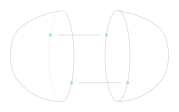
\includegraphics[width=0.75\textwidth]{images/clutching.png}};
		\node at(0.3,0) {$M\times$};
		\node at(5.9,0) {$\times M$};
		\node at(1.7,0.7) {$s$};
		\node at(2.3,-0.8) {$s'$};
		\node at(2.9,1) {$\varphi_s$};
		\node at(3.2,-0.5) {$\varphi_{s'}$};		
	\end{tikzpicture}
	\end{center}
	\end{minipage}
	\begin{minipage}[m]{0.35\textwidth}
		$\leadsto$ $\phi\colon M\times S^k\to M\times S^k$
		\[\phi(x,s) \coloneqq (\varphi_s(x),s) \]\pause
		\vspace{-1em}
		\[E\coloneqq M\times D^{k+1}\underset{\phi}{\cup} M\times D^{k+1}\]
		\vspace{-1em}
	\end{minipage}
	\vspace{-8.4em}
	}\pause
	\begin{prop}
		If $E$ is $\Spin$ and  \tikz[baseline]{
            \node[anchor=base] (s2)
            {$\ahat(E)$};
        } $\not=0$, then $[\varphi_s^*g]\not=0\in\pi_k(\calR^+(M))$.
	\end{prop}
	\vspace{-2em}
	\pause\pause
	\begin{center}
	\onslide<7->{
	\begin{tikzpicture}
		\node (s) at (-2.6,0.9) {};
		\node (t) at (-3.5,0.1) {};
		\node at (0,0) {$\coloneqq\scpr{\hat A(TE),[E]}\in\bbZ\quad \text{ for } \hat A $ a polynomial in Pontryagin classes}; 
		\draw[->, line width=1pt, bend right=20] (s) to (t);
	\end{tikzpicture}}\\
\onslide<8->{$\leadsto$ Are there $M$-bundles $E\to S^{k+1}$ with $E$ $\Spin$ and $\ahat(E)\not=0$?}
\end{center}
%	\renewcommand\CancelColor{\color{cyan}}
%	\only<6->{
%	\begin{prop}[Folklore]
%		$\begin{matrix} E \text{ admits \onslide<5->{\textcolor{cyan}{no}}}\\ \text{positive scalar curvature}\end{matrix}$ \qquad\only<-4>{$\Leftarrow$}\only<5->{\textcolor{cyan}{$\Rightarrow$}}\qquad $[f_s^*g]\only<-4>{=}\only<5->{\ \cancel=\ }0\in\pi_k(\calR^+(M))$.
%	\end{prop}\pause\pause
%	\begin{que}
%	What are obstructions to positive scalar curvature?\pause
%	\end{que}
%	\ \\
% 	\ \\
%	}
\end{frame}

\begin{frame}[plain]
\frametitle{Non-Rigidity of the action}
\topline
\begin{center}
$\leadsto$ Are there $M$-bundles $E\to S^{k+1}$ with $E$ $\Spin$ and $\ahat(E)\not=0$?\pause
	\end{center}
\begin{thm}[Hanke--Schick--Steimle, Wiemeler, Krannich--Kupers--Randal-Williams]\pause
\begin{enumerate}
	\item Such bundles exist (HSS).\pause
	\item If $p_i(TM)=0$ for all $i$ (HSS) or if $k>2\dim(M)$ (Wie), then $\ahat(E)=0$.\pause
	\item There exists a bundle $\mathbb{HP}^2\to E\to S^4$ with $\ahat(E) \not=0$ (KKRW).\pause
\end{enumerate}
\end{thm}
\begin{thm}[F. 2021]
	Assume, that $M$ is simply connected, $\Spin$ and $p_i(TM)\not=0$ for some $i$ and $k\le\min\left(\frac{\dim(M)-1}{3},\frac{\dim(M)-5}{2}\right)$. \\\pause
	Then there exists an $M$-bundle $E\to S^{k+1}$ with $E$ $\Spin$ and $\ahat(E)\not=0$.\\
\end{thm}
\end{frame}

\begin{frame}[plain]
\frametitle{{Non-Rigidity of the action}}
\topline	
\begin{thm}[F. 2021]
	Assume, that $M$ is simply connected, $\Spin$ and $p_i(TM)\not=0$ for some $i$ and $k\le\min\left(\frac{\dim(M)-1}{3},\frac{\dim(M)-5}{2}\right)$. \\
	Then there exists an $M$-bundle $E\to S^{k+1}$ with $E$ $\Spin$ and $\ahat(E)\not=0$.\\
\end{thm}\pause
\begin{remark}
	\begin{itemize}
		\item[-] $M$ as above $\leadsto$  $\pi_k(\calR^+(M))$ contains an element of infinite order.\pause
		\item[-] Examples of manifolds as in the theorem:
		\begin{itemize}
			\item $\mathbb{CP}^{2n+1}$, $\mathbb{HP}^{n}$, $\mathbb{OP}^{2}$ $\leadsto$ $\psec, \prc$\pause
			\item $n\ge2$: $S^n\times K3$\pause
			\item closed under products and connected sums with (almost) \emph{anything}\pause
		\end{itemize}
	\end{itemize}
	\qquad\qquad\alert{\large$\leadsto$ $\diff(M)\actson\calR^+(M)$ is often nontrivial!}\\\pause
	\begin{center}
	$\leadsto$ More Generally: Complete classification of monomial Pontryagin numbers for fiber bundles over spheres!
	\end{center}
\end{remark}
\end{frame}

\begin{frame}[plain]
\frametitle{What else is there to find in $\pi_k(\calR^+(M))$?}
\topline\\
\begin{thm}[F. 2021]
	Assume, that $M$ is simply connected, $\Spin$ and $p_i(TM)\not=0$ for some $i$ and $k\le\min\left(\frac{\dim(M)-1}{3},\frac{\dim(M)-5}{2}\right)$. \\
	Then $\pi_k(\calR^+(M))$ contains an element of infinite order.
\end{thm}\pause
\vspace{1em}
\begin{thm}[F.-Reinhold 2020]
	Let $n\ge5$, and let $M^{2n}$ be $\Spin$.\pause \\Then $\pi_k(\calR^+(M\#(S^n\times S^n)))$ is infinite for some $1\le k\le 9$.
\end{thm}\pause
\vspace{0.6em}
\only<1-6>{
\begin{remark}
\begin{itemize}
	\item[-] Also generalizes to $\calR_C(M\#(S^n\times S^n))\subset\calR^+(M\#(S^n\times S^n))$.\pause
	\item[-] Version for odd dimensions.\pause
	\item[-] Proof: Construct $M\#(S^n\times S^n)$-bundles $E\to S^a\times S^b$ with $\ahat(E)\not=0$.
	\item
\end{itemize}
\end{remark}}
\pause\pause\pause
\only<7-10>{
\begin{exampleblock}{Future Projects}
\begin{itemize}\item\begin{itemize}\pause
	\item Explore other methods to construct and distinguish (families of) metrics.\pause
	\item Study a simplicial approximation of $\calR^+(M)$ and find upper bounds on the homotopy type. \pause
	\item Study (spaces of) metrics with symmetries.
	\vspace{1em}
\end{itemize}\end{itemize}
\end{exampleblock}

}
\end{frame}

\begin{frame}[plain]
\frametitle{Rigidity of the action and multiplicative structure}
\topline
\pause
	\begin{thm}[F. 2019]
		Let $\dim(M)\ge6$ and $\varphi$ be a diffeomorphism of $M$ such that\\ $T_\varphi$ \onslide<3->{ is nullbordant in the tangential $2$-type of $M$. Then $\varphi^*\sim id$.}
	\end{thm}
	\only<2>{
	\begin{tikzpicture}
		\node at (4,0) {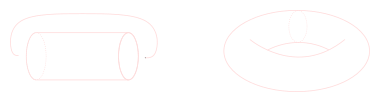
\includegraphics[width=1\textwidth]{images/mapping torus.pdf}};
		\node at (0.8,1.3) {$\varphi$};
		\node at (4,0){$\leadsto$};
		\node at (7.2,1.4) {$\varphi$};
		\node at (4.8,-0.6) {\large $T_\varphi$};
	\end{tikzpicture}
	\vspace{-10.6em}
	}\pause\pause
	\begin{cor}
		If $\dim(M)=6$ and $M$ is simply connected, then  $T_\varphi$ is nullbordant in the tangential $2$-type of $M$ for every diffeomorphism $\varphi\colon M\to M$.
	\end{cor}\pause

	\only<1-7>{\begin{example}[Further manifolds this is applicable to]\pause
		\begin{itemize}
			\item[$>$] homotopy spheres, stably parallelizable manifolds in $\dim\not=0,1(8)$\pause
			\item[$>$] closed under products and connected sums.
		\end{itemize}	
	\end{example}\pause}
	\begin{thm}[F. 2020]
		If $\dim(M)\ge6$ and $M$ is nullbordant in its own tangential $2$-type (e.g. if $M=N\times S^2$), then $\calR^+(M)$ is a homotopy-commutative, homotopy-associative $H$-space.
	\end{thm}
	\only<8-10>{\pause\pause\pause\pause
\begin{exampleblock}{Future Projects}
\begin{itemize}\item\begin{itemize}
	\item \dots\pause
	\item Rigidity of the action $\diff(M)\actson\calR^+(M)$ on $\pi_k$ for $k\ge1$\vspace{1em}
\end{itemize}\end{itemize}
\end{exampleblock}
}
\end{frame}


\begin{frame}[plain]
\centering
\vspace{2em}
\huge Thank you!
\vspace{1em}
\begin{exampleblock}{Future Projects}
\vspace{0.3em}
\begin{itemize}
\item\begin{itemize}
	\item Explore other methods to construct (families of) metrics.\vspace{1em}
	\item Study a simplicial approximation of $\calR^+(M)$ and find upper bounds on the homotopy type.\vspace{1em}
	\item Study (spaces of) metrics with symmetries.\vspace{1em}
	\item Rigidity of the action $\diff(M)\actson\calR^+(M)$ on $\pi_k$ for $k\ge1$.
\end{itemize}
\end{itemize}
\end{exampleblock}
\end{frame}

\end{document}





